\section{Analiza wymagań}
Przed implementacją systemu należy przeprowadzić analizę problemu, określić wymagania systemu, zadecydować o narzędziach i technologiach niezbędnych w implementacji systemu.
W tym rozdziale zostanie najpierw opisany problem oraz koniecznie do zaimplementowania moduły, następnie postawione zostaną wymagania jakie system musi spełniać. Ostatnim krokiem będzie omówienie narzędzi i technologii koniecznych do implementacji systemu.
\subsection{Opis problemu}
\begin{par}
	Tematem pracy jest zaprojektowanie i implementacja systemu podejmującego decyzje w prostej grze platformowej czasu rzeczywistego.
	Moduł odpowiedzialny za optymalizację przejścia gry, oraz podejmowanie akcji powinien być oparty o zagadnienie algorytmów genetycznych.
	Celem samej gry jest dotarcie do zdefiniowanego wcześniej celu na dwuwymiarowej mapie. Wynik końcowy przejścia może zależeć od wielu parametrów - mapa może zawierać elementy dające punkty, jak i elementy prowadzące do natychmiastowego zakończenia gry (z wynikiem pozytywnym bądź negatywnym).
	Efektem pracy powinien być system pozwalający na rozwiązanie tego typu problemu bazujący na algorytmie genetycznym.
	\newline
	Ogólne wymogi dotyczące systemu:
	\begin{itemize}
		\item
			System powinien składać się z bazowego silnika gry, wzorowanego na rozwiązaniach w klasycznych grach platformowych. Ma to być jednocześnie warstwa prezentacyjna algorytmu.
			System nie powinien sztywno zakładać realizacji algorytmu na konkretnej grze platformowej, lecz być ogólnym systemem rozwiązującym gry platformowe czasu rzeczywistego.
		\item
			System powinien pozwalać zarówno na poruszanie się po mapie przez użytkownika jak i przejście w tryb treningu populacji, który na podstawie zadanych parametrów optymalizuje przejście po mapie algorytmem genetycznym.
		\item
			Do wyniku końcowego mogą być brane pod uwagę również inne zdarzenia takie jak ilość zebranych obiektów na planszy, czy czas przejścia gry.
			Funkcja przystosowania zależeć będzie od rożnych czynników, a ich modyfikacja powinna być łatwo dostępna.
		\item
			Projekt ma mieć charakter edukacyjno-badawczy. Przydatnymi narzędziami w systemie będzie prosty w obsłudze edytor map, panel konfiguracyjny w którym możemy edytować większość parametrów związanych z samym działaniem algorytmu oraz aktywny podgląd populacji i osobników.
	\end{itemize}
\end{par}

\begin{par}
	Sam pomysł stworzenia sztucznej inteligencji do gry platformowej w czasie rzeczywistym został już wcześniej powoływany do życia, m.in. jako projekt MarioAI. 
	W chwili obecnej funkcjonuje on jako turniej dla programistów. 
	Uczestnicy mogą implementować własne rozwiązania do gotowego silnika generującego losowe poziomy, oraz porównywać wyniki z innymi uczestnikami.
	Samo zgłoszenie składa się z implementacji własnej klasy odpowiedzialnej za podejmowanie decyzji.
	Strona domowa projektu znajduje się pod adresem www.marioai.org.
\end{par}

\subsection{Wymagania funkcjonalne}
	System nie wymaga różnicowania użytkowników ze względu na role. Wymagania funkcjonalne wyglądają następująco:
	\begin{itemize}
		\item {\bf Poruszanie się w środowisku gry za pomocą klawiatury.}
		\newline
		Podstawowym wymogiem systemu jest implementacja silnika prostej gry platformowej pozwalającego na poruszanie się postacią po mapie.
		Sterowanie zrealizowane powinno być intuicyjne i analogiczne do przyjętych rozwiązań w grach platformowych.
		Ponieważ oprawa graficzna nie jest priorytetem w projekcie, wystarczy prosta reprezentacja obiektów za pomocą prostokątów.
		\item {\bf Wczytanie mapy do środowiska gry.}
		\newline
		System powinien pozwalać na wczytywanie map z plików tekstowych do bieżącego środowiska symulującego przebieg gry.
		Wówczas bieżąca gra zostaje przerwana i inicjowany jest nowy przebieg gry na nowowczytanej mapie.
		\item {\bf Wczytanie nowej logiki do środowiska gry.}
		\newline
		Ponieważ system powinien być ogólnym systemem rozwiązującym gry platformowe, dostępnych powinno być kilka przykładowych gier,
		różniących się między sobą pod względem logiki. Podobnie jak w powyższym przypadku bieżąca gra powinna zostać przerwana i
		powinien zostać zainicjowany nowy przebieg gry z nową logiką.
		\item {\bf Przejście w tryb treningu populacji.}
		\newline
		Po przejściu w tryb treningu populacji użytkownikowi odbierana jest możliwość poruszania się postacią po ekranie.
		Jeśli nie istnieje jeszcze zainicjowana żadna populacja początkowa, następuje wylosowanie pierwszej populacji, po czym system rozpoczyna trening populacji w danym środowisku gry, zgodnie z danymi ustawieniami w systemie. Przechodzenie pomiędzy treningiem populacji a grą użytkownika powinno być możliwe w obie strony. 
		Wówczas jeśli użytkownik zainicjuje trening populacji, następnie przejdzie w tryb swobodnej gry, a ostatecznie znowu rozpocznie trening populacji, domyślną populacją jest ta która została zapisana podczas ostatniego treningu.
		\item {\bf Zainicjowane nowej populacji. }
		\newline
		Może okazać się koniecznie zainicjowanie nowej populacji podczas działania systemu, np. gdy populacja wpadła w stagnację.
		Inicjowanie nowej populacji podczas zmiany logiki, ustawień bądź wczytywania mapy jest realizowane automatycznie.
		\item {\bf Otworzenie okna ustawień.}
		\newline
		System ze względu na warstwę genetyczną powinien być w łatwo konfigurowalny. Po wyświetleniu okna ustawień użytkownik ma możliwość zmiany
		poszczególnych parametrów algorytmu bądź symulacji gry.
		\item {\bf Zastosowanie nowych ustawień. }
		\newline
		Ponieważ niektóre ustawienia wymagają porzucenia aktualnego wyniku populacji i rozpoczęcia symulacji od początku (np. rozmiar chromosomu).
		Użytkownik jest o tym fakcie informowany i pytany o ponownie uruchomienie algorytmu. 
		W przypadku gdy nie jest to koniecznie, algorytm nie zostaje przerwany, a użytkownik wedle woli może to uczynić własnoręcznie.
		\item {\bf Otworzenie okna populacji. }
		\newline
		Podczas działania algorytmu powinien być możliwy podgląd aktualnej populacji. Użytkownikowi widoczna jest wówczas lista osobników, oraz krótki opis każdego z nich:
		Wynik końcowy, ilość zebranych punktów, czas działania, wartość funkcji przystosowania. Dodatkowym elementem jest możliwość przerwania aktualnego przebiegu gry i uruchomienie tymczasowo nowego przebiegu dla dowolnego osobnika z listy wybranego przez użytkownika. Po zakończeniu przebiegu algorytm powraca do treningu populacji.
		\item {\bf Otworzenie okna osobnika. }
		\newline
		Bezpośrednio z okna populacji użytkownik ma możliwość podejrzenia szczegółów dotyczących osobników. Wówczas otwierane jest nowe okno zawierające wszystkie informacje na temat danego osobnika takie jak długość tablicy chromosomu bądź tekstowa reprezentacja całego chromosomu.
		\item {\bf Otworzenie okna edytora map. }
		\newline
		Ważnym elementem systemu jest narzędzie pozwalające tworzyć nowe mapy oraz modyfikować istniejące.
		Użytkownik po otworzeniu okna edytora map ma do dyspozycji narzędzia pozwalające na umieszczanie prostokątnych obiektów na planszy odpowiadających za typy obiektów występujących w grze. Oprócz tego niezbędne są narzędzia edycji takie jak cofnięcie ostatniej akcji, usunięcie wszystkich obiektów, bądź zaznaczanie poszczególnych.
		\item {\bf Wczytywanie oraz Zapisywanie map do edytora. }
		\newline
		Wczytywanie może być zrealizowane analogicznie do wczytywania mapy do środowiska gry. Podobnie zapis mapy powinien być dostępny dla użytkownika z menu, dzięki czemu informacje o aktualnie tworzonej mapie są dostępne do wczytania przez silnik gry.
		\item {\bf Przyspieszenie pracy algorytmu.}
		\newline
		Podczas treningu populacji często niepotrzebne jest użytkownikowi śledzenie ruchów algorytmu szczególnie w początkowym stadium. Aby szybciej osiągnąć wyniki działania algorytmu rozgrywka jest przyspieszana przez wstrzymanie wyświetlania grafiki na mapie. Oprócz tego opóźnienie koniecznie do osiągnięcia 60 klatek na sekundę podczas wyświetlania zostaje wyłączone - algorytm w tle przeprowadza symulacje.
	\end{itemize}
\subsection{Wymagania niefunkcjonalne}
	\begin{enumerate}
	\item {\bf Prędkość działania aplikacji. }	
	\newline
	Ponieważ aplikacja wymaga przeprowadzenia wielu symulacji gry do osiągnięcia wyniku, koniecznie jest optymalne zaprojektowanie funkcji biorących udział w działaniu algorytmu genetycznego.
	\item {\bf Elastyczność. }
	\newline
	System powinien być napisany w taki sposób aby możliwe było go późniejsze rozwijanie, szczególnie jeśli chodzi o rozszerzanie systemu o nowe logiki gier.
	System musi zostać rozpatrzony jako generalny system rozwiązujący gry czasu rzeczywistego opierające się na 4 klawiszach kierunkowych i do 4 klawiszy specjalnych.
	\item {\bf Oprawa Graficzna. }
	\newline
	Oprawa graficzna samej gry nie jest istotna w systemie. Jeśli system ma być elastyczny jeśli chodzi o mechanikę gier, wprowadzenie bogatej grafiki niepotrzebne skomplikuje proces dodawania nowego typu gry do systemu. 
	Innym powodem zachowania prostej grafiki jest swoboda rozmiarów obiektów. 
	W większości gier platformowych stosowana jest grafika rastrowa która przy skalowaniu obiektów bez zachowania proporcji wygląda źle.
	Rozwiązanie tego problemu wiązałoby się z generowaniem grafiki proceduralnie bądź używaniem grafiki wektorowej, co jednak odbiega od istoty pracy.
	\end{enumerate}

\subsection{Wykorzystane narzędzia i języki programowania}
\begin{par}
	Głównym celem do zrealizowania w pracy jest problem algorytmiczny i teoretyczny.
Praca w mniejszym stopniu opiera się na wykorzystaniu konkretnej technologii, czy języka programowania, wobec czego zostały wykorzystane popularne narzędzia i języki programowania.
Językiem programowania wykorzystanym w aplikacji jest język java.
Ponieważ część algorytmiczna aplikacji wymaga przeprowadzania częstych symulacji zachowania środowiska oraz przeprowadzania całego przebiegu gry, istotnym czynnikiem był czas działania krytycznych miejsc w aplikacji - głównie pętli gry, wyświetlania oraz generowania nowej populacji na podstawie poprzedniej.
Java jako język polegający na maszynie wirtualnej posiada warstwę pośrednią która spowalnia cały proces jest wolniejsza od języka C lub C++,
jednak prostota realizacji części wizualnej aplikacji, bardzo dobra przenośność języka java oraz relatywnie małe zyski czasowe przeważyły w wyborze języka.
Kolejnym trafnym wyborem jeśli chodzi o język i narzędzia byłby prawdopodobnie C++ wraz z biblioteką Qt do generowania grafiki i tworzenia okienek oraz kontrolek.
Tą samą aplikację można by zrealizować za pomocą języka Python i biblioteki PyGame do warstwy wizualizacyjnej,
jednak wówczas koszt czasowy realizacji algorytmu genetycznego oraz logiki gry mógłby okazać się znacząco duży, ze względu na fakt iż Python jest językiem interpretowanym, i generalnie nie jest przeznaczony do dużych i częstych obliczeń.
Przy konieczności realizacji prostej wersji demonstracyjnej programu opisywanego w pracy, język Python wraz z biblioteką PyGame może okazać się najszybszym do implementacji ze względu na krótki kod, dynamiczne typy zmiennych oraz bogatą kolekcję struktur takich jak listy czy mapy incydencji konieczne do realizacji algorytmu.
Sama aplikacja korzysta z kolekcji i podstawowych struktur danych występujących w języku Java.
Warstwa graficzna korzysta z biblioteki Swing do rysowania interfejsu użytkownika oraz AWT do reakcji na zdarzenia.
Inną biblioteką wykorzystywaną do tworzenia graficznych interfejsów użytkownika jest SWT, która nie tylko jest równie przenośnia, lecz też imituje wygląd domyślnie używany w systemie operacyjnym - aplikacje napisane w całości w Swing wyglądają tak samo bez względu na system operacyjny.
Aplikacja w całości została zrealizowana w programie Netbeans 6.9.1 wspierającym testowanie, kompilację budowanie aplikacji napisanych w języku Java.
Innym popularnym narzędziem może być Eclipse, jednak lepsze narzędzia testujące (ang. profiler) przeważyły o wyborze pierwszej aplikacji.
\end{par}
\subsection{Diagram przypadków użycia}
\begin{par}
	Diagram przypadków użycia został przedstawiony na Rys. \ref{fig:diagram_przypadkow}.
		\begin{figure}[!h]
		\centering
		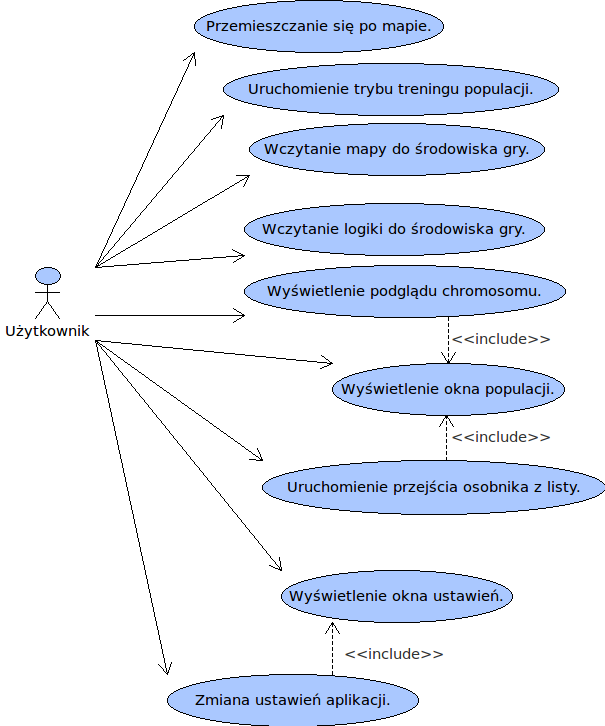
\includegraphics[width=\textwidth]{obrazki/diagram_przypadkow.png}
		\caption{Diagram przypadków użycia.}
		\label{fig:diagram_przypadkow}
		\end{figure}
		\FloatBarrier
\end{par}
\subsection{Opis tekstowy przypadków użycia}
\begin{par}
	We wszystkich przypadkach użycia aktorem jest użytkownik aplikacji.
	\begin{itemize}

	\item
	Opis przypadku użycia {\bf Przemieszczanie się po mapie }.
	\begin{enumerate}
	\item Podstawowy ciąg zdarzeń:
		\begin{enumerate}
		\item Po uruchomieniu instancji gry w głównym oknie aplikacji wyświetlona zostaje mapa wraz ze znajdującymi się na niej obiektami.
		\item Użytkownik za pomocą klawiszy na klawiaturze przesyła dane dotyczące ruchu i akcji specjalnych do środowiska gry.
		\item Postać gracza znajdująca się w grze reaguje na żądane akcje, logika gry decyduje o reakcjach obiektów w środowisku na postępy gracza.
		\item Gracz wchodzi w kolizję z jednym z obiektów kończących grę z danym wynikiem pozytywnym bądź negatywnym.
		\item Po zakończeniu gry mapa jest ponownie wczytywana i automatycznie rozpoczynana jest nowa instancja gry.
		\end{enumerate}
	\item Alternatywne ciąg zdarzeń:
		\begin{enumerate}
		\item Użytkownik w trakcie gry uruchamia tryb treningu populacji.
		\item Użytkownik w trakcie gry wczytuje nową mapę, bądź nową logikę gry, przez co gra jest przerywana i rozpoczynana od nowa.
		\end{enumerate}
	\item Zależności czasowe:
		\begin{enumerate}
		\item Częstotliwość wykonania: Samo przemieszczanie się po mapie jest akcją o charakterze ciągłym. 
		Rozpoczynanie akcji poruszania się po mapie ze stanu treningu populacji jest bliżej nieokreślone, lecz może być wykonywane średnio 1-2 razy na minutę działania aplikacji.
		\item Typowy czas realizacji: 1 minuta.
		\item Maksymalny czas realizacji: nieokreślony.
		\end{enumerate}
	\item Wartości uzyskiwane przez aktorów po zakończeniu przypadku użycia:
		\begin{enumerate}
		\item Jeśli użytkownik zakończy tryb poruszania się po mapie przez przełączenie na tryb treningu populacji, wówczas traci kontrolę nad postacią i nie ma wpływu na akcje rozgrywane w środowisku gry.
		\end{enumerate}
	\end{enumerate}
	\item
	Opis przypadku użycia {\bf Uruchomienie trybu treningu populacji. }.
	\begin{enumerate}
	\item Podstawowy ciąg zdarzeń:
		\begin{enumerate}
		\item Podczas działania aplikacji gracz uruchamia tryb treningu populacji.
		\item Jeśli jest to pierwsze uruchomienie trybu treningu wówczas nie istnieje wcześniejsza populacja, wówczas losowana jest populacja początkowa. W przeciwnym wypadku, symulacja zaczyna się od ostatniej populacji wygenerowanej przez system. 
		\item System kolejno przeprowadza wszystkie kroki algorytmu genetycznego na bieżącej populacji.
		\item Jeśli wyświetlone jest okno widoku populacji jest ono aktualizowane po każdym przebiegu gry.
		\end{enumerate}
	\item Alternatywne ciąg zdarzeń:
		\begin{enumerate}
		\item Użytkownik wybiera w oknie populacji osobnika i przeprowadza jego tymczasową symulację w środowisku, przez co trening jest chwilowo wstrzymany. Po symulacji gry danego osobnika trening jest wznawiany od ostatniego osobnika.
		\item Użytkownik wczytuje nową logikę bądź mapę, przez co aktualny przebieg gry jest przerywany. Zostaje uruchomiona nowa gra i trening populacji jest automatycznie uruchamiany od początku.
		\item Użytkownik zmienia ustawienia algorytmu genetycznego. Jeśli są to zmiany wymagające ponownego uruchomienia gry jest wyświetlony komunikat potwierdzający operację, w innym wypadku zmiany następują bez zaburzania aktualnego przebiegu treningu.
		\item Użytkownik uruchamia tryb przyspieszonego treningu, przez co wyłączona zostaje aktualizacja stanu gry w oknie aplikacji.
		\end{enumerate}
	\item Zależności czasowe:
		\begin{enumerate}
		\item Częstotliwość wykonania: Przełączanie na trening populacji może być średnio uruchamiane 1-2 razy w ciągu minuty działania aplikacji. 
		\item Typowy czas realizacji: 10 sekund - 5 minut. Samo działanie treningu populacji stanowić może około 90\% czasu działania aplikacji.
		\item Maksymalny czas realizacji: nieokreślony.
		\end{enumerate}
	\item Wartości uzyskiwane przez aktorów po zakończeniu przypadku użycia:
		\begin{enumerate}
		\item Jeśli użytkownik uruchomi tryb poruszania się po mapie wówczas przywrócone zostaje wyświetlanie stanu gry (jeśli był włączony tryb przyspieszonego treningu). Użytkownik uzyskuje kontrolę nad postacią gracza.
		\end{enumerate}
	\end{enumerate}
	\item
	Opis przypadku użycia {\bf Edycja bieżącej mapy. }.
	\begin{enumerate}
	\item Podstawowy ciąg zdarzeń:
		\begin{enumerate}
		\item Użytkownik klika w przycisk menu dotyczący edytora map.
		\item Wyświetlone zostaje nowe okno aplikacji zawierające przyciski dotyczące edycji mapy.
		\item Do edytora map domyślnie zostaje wczytana bieżąca mapa wczytana do środowiska symulatora.
		\item Użytkownik wybiera obiekty gry użyciu przycisków znajdujących się w menu okna a następnie metodą przeciągnij-upuść rysuje prostokątne obiekty odpowiadające za obiekty w grze.
		\item Użytkownik z menu wybiera opcję zapisu mapy do pliku.
		\item Wyświetlone zostaje okno dialogowe zapisu pliku w którym użytkownik wybiera nazwę pliku.
		\item Użytkownik zamyka okno edytora map.
		\end{enumerate}
	\item Alternatywne ciąg zdarzeń:
		\begin{enumerate}
		\item Użytkownik wczytuje nowa mapę do edytora map. 
			\begin{enumerate}
			\item Wyświetlone zostaje okno dialogowe dotyczące otwarcia pliku z systemu.
			\item Wszystkie obiekty z planszy zostają usunięte, i wczytywane są nowe z wybranej wcześniej mapy.
			\end{enumerate}
		\end{enumerate}
	\item Zależności czasowe:
		\begin{enumerate}
		\item Częstotliwość wykonania: 0-5 razy w ciągu działania aplikacji.
		\item Typowy czas realizacji: 5 minut.
		\item Maksymalny czas realizacji: nieokreślony.
		\end{enumerate}
	\item Wartości uzyskiwane przez aktorów po zakończeniu przypadku użycia:
		\begin{enumerate}
		\item Użytkownik po zapisaniu stworzonej mapy do pliku ma możliwość wczytania mapy z dysku do symulatora gry i przeprowadzenia treningu populacji na nowej mapie.
		\end{enumerate}
	\end{enumerate}
	\item
	Opis przypadku użycia {\bf Zmiana ustawień aplikacji. }.
	\begin{enumerate}
	\item Podstawowy ciąg zdarzeń:
		\begin{enumerate}
		\item Użytkownik wyświetla okno ustawień aplikacji.
		\item W polach tekstowych użytkownik dokonuje zmian na poszczególnych parametrach aplikacji
		\item Użytkownik zatwierdza zmiany przyciskiem.
		\item System sprawdza czy zmiany nie wymagają przerwania bieżącej gry i ponownego uruchomienia algorytmu.
		\begin{enumerate}
			\item Jeśli zmiany nie wymagają ponownego uruchomienia algorytmu, zmiany zostają wprowadzone bez przerywania bieżącej instancji gry.
			\item W wypadku gdy ponowne uruchomienie jest koniecznie wyświetlone zostaje okno dialogowe.
			Użytkownik jest pytanie o ponowne uruchomienie algorytmu, ma wówczas on do dyspozycji zgodę na operację, bądź cofnięcie zmian wymagających ponownego uruchomienia.
			\item Po podjęciu decyzji okno dalej pozostaje otwarte, a zgodnie z wyborem zmiany zostają dokonane bądź nie.
		\end{enumerate}
		\item Użytkownik dalej może dokonywać zmian ustawieniach aplikacji.
		\end{enumerate}
	\item Alternatywne ciąg zdarzeń:
		\begin{enumerate}
		\item Użytkownik dokonuje zmian, lecz zamiast zatwierdzić je przyciskiem - zamyka okno ustawień. Wówczas po ponownym otwarciu ładowane są aktualne ustawienia a zmiany wprowadzone przez użytkownika nie są zapamiętywane.
		\end{enumerate}
	\item Zależności czasowe:
		\begin{enumerate}
		\item Częstotliwość wykonania: 0-5 razy w ciągu działania aplikacji.
		\item Typowy czas realizacji: 1 minuta.
		\item Maksymalny czas realizacji: nieokreślony.
		\end{enumerate}
	\item Wartości uzyskiwane przez aktorów po zakończeniu przypadku użycia:
		\begin{enumerate}
		\item brak
		\end{enumerate}
	\end{enumerate}

	\item
	Opis przypadku użycia {\bf Wyświetlenie podglądu populacji. }.
	\begin{enumerate}
	\item Podstawowy ciąg zdarzeń:
		\begin{enumerate}
		\item Podczas treningu populacji użytkownik z menu w oknie głównym gry wybiera opcję ``Population''.
		\item Okno zostaje wyświetlone, i utworzony zostaje komponent JList wypełniony aktualnymi osobnikami z populacji.
		\item Jeśli dany osobnik na liście już przeprowadził symulację, widoczne są wartości punktowe zdobyte przez danego osobnika, czas przejścia oraz wynik końcowy.
		\item Podczas działania algorytmu lista jest automatycznie aktualizowana.
		\item Użytkownik zamyka okno populacji.
		\end{enumerate}
	\item Alternatywne ciąg zdarzeń:
		\begin{enumerate}
		\item Użytkownik zaznacza osobnika i wyświetla o nim szczegóły.
		\begin{enumerate}
			\item Uruchamiany jest przypadek użycia ``Wyświetlenie podglądu chromosomu''.
		\end{enumerate}
		\item Użytkownik zaznacza osobnika i uruchamia jego przejście gry.
		\begin{enumerate}
			\item Uruchamiany jest przypadek użycia ``Uruchomienie przejścia osobnika z listy.''.
		\end{enumerate}
		\end{enumerate}
	\item Zależności czasowe:
		\begin{enumerate}
		\item Częstotliwość wykonania: 0-5 razy w ciągu działania aplikacji.
		\item Typowy czas realizacji: 1 minuta.
		\item Maksymalny czas realizacji: nieokreślony.
		\end{enumerate}
	\item Wartości uzyskiwane przez aktorów po zakończeniu przypadku użycia:
		\begin{enumerate}
		\item brak
		\end{enumerate}
	\end{enumerate}
	\item
	Opis przypadku użycia {\bf Wyświetlenie podglądu chromosomu. }.
	\begin{enumerate}
	\item Podstawowy ciąg zdarzeń:
		\begin{enumerate}
		\item Użytkownik zaznacza osobnika z listy w oknie populacji.
		\item Przyciskiem "Show details" wyświetla okno szczegółów na temat danego osobnika.
		\item Dane na temat osobnika są w postaci tekstowej - użytkownik może je skopiować do schowka.
		\item Użytkownik zamyka okno szczegółów.
		\end{enumerate}
	\item Alternatywne ciąg zdarzeń:
		\begin{enumerate}
		\item Użytkownik otwiera okna szczegółów dla kilku osobników po kolei - Otwiera się kilka osobnych okien.
		\end{enumerate}
	\item Zależności czasowe:
		\begin{enumerate}
		\item Częstotliwość wykonania: 0-5 razy w ciągu działania aplikacji.
		\item Typowy czas realizacji: 20 sekund.
		\item Maksymalny czas realizacji: nieokreślony.
		\end{enumerate}
	\item Wartości uzyskiwane przez aktorów po zakończeniu przypadku użycia:
		\begin{enumerate}
		\item brak.
		\end{enumerate}
	\end{enumerate}

	\item
	Opis przypadku użycia {\bf Uruchomienie przejścia osobnika z listy. }.
	\begin{enumerate}
	\item Podstawowy ciąg zdarzeń:
		\begin{enumerate}
		\item Użytkownik zaznacza osobnika z listy w oknie populacji.
		\item Przyciskiem "Run selected" zatwierdza wybór osobnika.
		\item Jeśli jest aktualnie przeprowadzana symulacja wówczas zostaje ona przerwana i rozpoczyna się przejście gry wybranego wcześniej osobnika.
		\item Po zakończeniu przejścia system ponownie wraca do treningu populacji i zaczyna od ostatniego osobnika.
		\end{enumerate}
	\item Alternatywne ciąg zdarzeń:
		\begin{enumerate}
		\item Użytkownik uruchamia przejście osobnika w trybie przemieszczania się po mapie. Symulacja nie zostaje wówczas przeprowadzona.
		\end{enumerate}
	\item Zależności czasowe:
		\begin{enumerate}
		\item Częstotliwość wykonania: 0-10 razy w ciągu działania aplikacji.
		\item Typowy czas realizacji: zależny od długości przejścia osobnika 1 - 40 sekund.
		\item Maksymalny czas realizacji: nieokreślony.
		\end{enumerate}
	\item Wartości uzyskiwane przez aktorów po zakończeniu przypadku użycia:
		\begin{enumerate}
		\item brak.
		\end{enumerate}
	\end{enumerate}

	\end{itemize}
\end{par}

\subsection{Diagramy czynności}
\begin{par}
		Poniżej zostaną przedstawione diagramy czynności najistotniejszych czynności w systemie.
		\begin{figure}[!h]
		\centering
		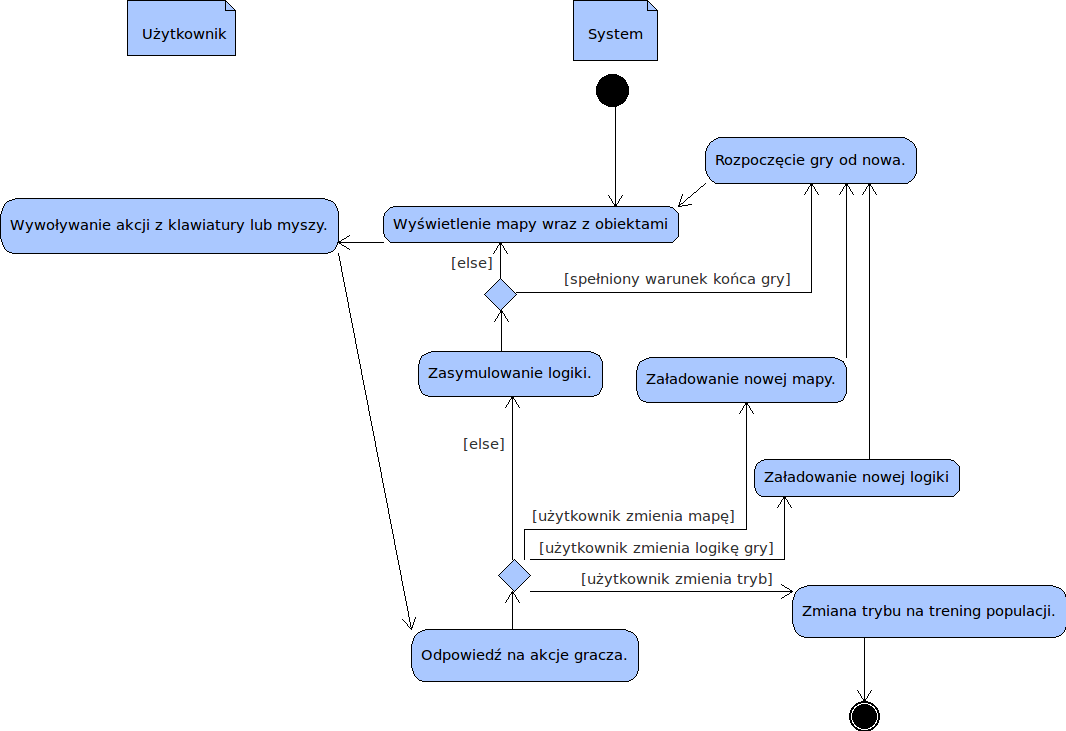
\includegraphics[width=\textwidth]{obrazki/activity_diagram.png}
		\caption{Diagram czynności ``Przemieszczanie się po mapie''.}
		\label{fig:sterowanie}
		\end{figure}
		\begin{figure}[!h]
		\centering
		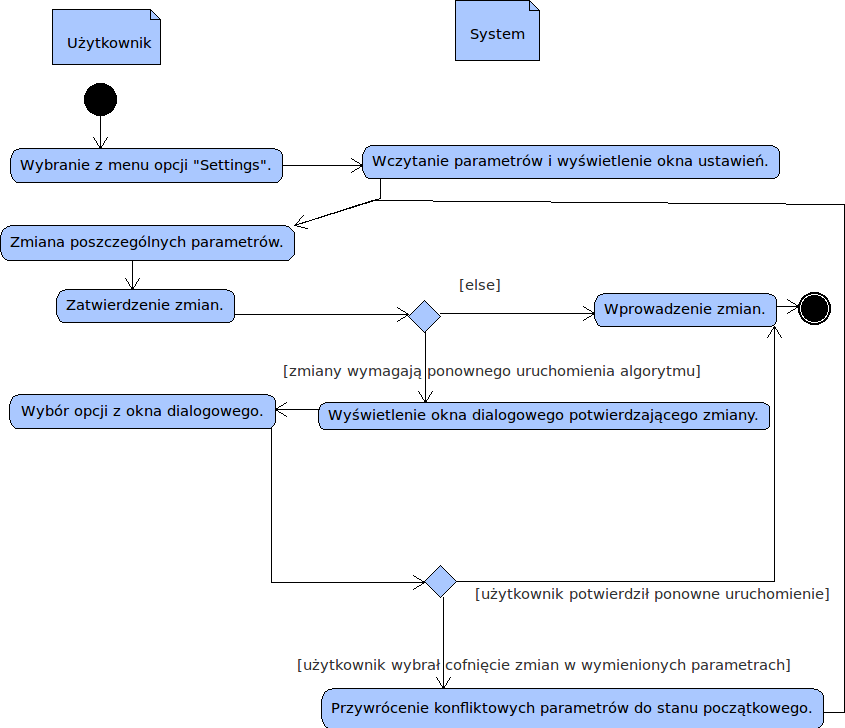
\includegraphics[width=\textwidth]{obrazki/activity_diagram_2.png}
		\caption{Diagram czynności ``Zmiana ustawień aplikacji''.}
		\label{fig:sterowanie}
		\end{figure}
		\begin{figure}[!h]
		\centering
		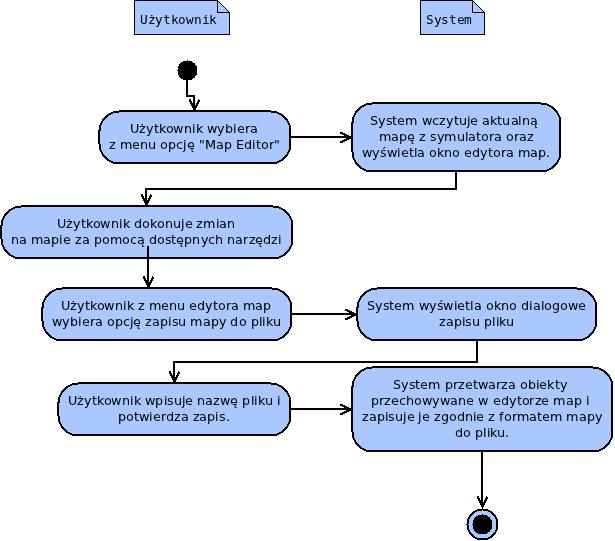
\includegraphics[width=\textwidth]{obrazki/czynnosci_edytor_map.jpeg}
		\caption{Diagram czynności ``Edycja bieżącej mapy''.}
		\label{fig:sterowanie}
		\end{figure}
		\FloatBarrier
\end{par}

\subsection{Wstępna analiza problemu}
\begin{par}
	\subsubsection{Sterowanie}
	\begin{par}
	Aby zrealizować część odpowiedzialną za sterowanie postacią, należy użyć klasy pośredniej pomiędzy warstwą logiki silnika gry, a warstwą komunikacji z graczem.
	Przy takim rozwiązaniu sygnały z klawiatury bądź innych urządzeń peryferyjnych są przekazywane do warstwy pośredniczącej.
	Dzięki takiemu wyjściu możemy łatwo zmienić źródło sygnałów trafiających do postaci z bezpośrednich wciśnięć klawiszy na akcje przechowywane w chromosomie.
	Warstwa pośrednia odpowiada wówczas za sterowanie postacią gracza w taki sam usystematyzowany sposób, niezależnie od źródła sygnałów. 
	Z punktu widzenia logiki gry nie ma różnicy pomiędzy sygnałami z klawiatury, a wygenerowanymi akcjami.
	\end{par}
	
	\subsubsection{Projekt chromosomu}
	Kolejnym ważnym elementem jest odpowiednie zaprojektowanie struktury chromosomu. 
	Dwa najbardziej trafne rozwiązania opierają się na dwóch zmiennych występujących w środowisku gry: czasie oraz pozycji gracza.
	\begin{enumerate}
	\item
	{\bf Czas który upłynął od rozpoczęcia danej instancji przejścia. }
	\begin{par}

		To rozwiązanie zakłada podejmowanie akcji w grze w zależności od czasu który upłynął od jej rozpoczęcia.
		Warto zauważyć iż nie jesteśmy ograniczeni położeniem postaci na planszy, dzięki czemu możliwe są takie operacje jak brak akcji, czy powrót do początku planszy jeśli to korzystne.
		Istotną wadą tego rozwiązania byłaby duża podatność algorytmu na zapętlanie się, lub wykonywanie dużej ilości mało przydatnych ruchów. 
		Można łatwo zauważyć że przy równym prawdopodobieństwie ruchu w lewo i prawo, postać tylko nieznacznie będzie oddalać się punktu startowego. 
		Prostym rozwiązaniem tego problemu jest przyporządkowanie pewnego prawdopodobieństwa każdej akcji, dzięki czemu możemy założyć że preferowanym kierunkiem jest np. ruch postaci w prawo, nie tracąc możliwości minimalnego ruchu w lewo jeśli to korzystne.
		Pewnym utrudnieniem może być krzyżowanie tego typu chromosomów. Ponieważ akcje postaci w większości przypadków mają sens w kontekście jej aktualnego położenia, o tyle klasyczne krzyżowanie poprzez ''cięcia'' chromosomu na dwie części może okazać się kosztowne.
		Wybranie losowego punktu przecięcia i złączenie ze sobą dwóch chromosomów nie jest dobrym rozwiązaniem.
		Po połączeniu otrzymamy niespójny ciąg ruchów, które będą miały niewiele wspólnego z aktualną pozycją gracza na mapie, wobec czego będą nieużyteczne.
		Można temu zapobiec zapewniając łączenie się chromosomów jedynie w punktach w których postać w obu momentach znajduje się w tym samym lub zbliżonym miejscu. Wyznaczenie takich punktów może okazać się kosztowne.
		Przeszukiwanie punktów wspólnych można zrealizować w czasie $O(n*log_2n)$ najpierw sortując tablice obu osobników odpowiadające za ruch w chromosomie. 
		Tablice sortujemy względem współrzędnej X aktualnego położenia gracza dla każdej z akcji, a następnie liniowo przechodząc po obu tablicach osobników, szukając punktów wspólnych.
		Wówczas widać iż trzeba przechowywać dane na temat położenia w chromosomie, co jest nieco niespójne z ideą poruszania się względem czasu.
		Wstępny schemat takiego rozwiązania mógłby wówczas wyglądać tak jak na rysunku \ref{fig:sterowanie}.
		
		\begin{figure}[!h]
		\centering
		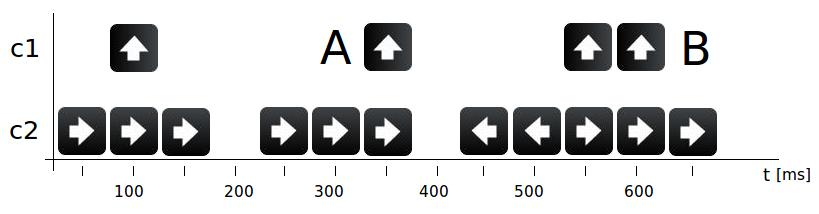
\includegraphics[width=\textwidth]{obrazki/sterowanie.jpg}
		\caption{Sterowanie względem czasu.}
		\label{fig:sterowanie}
		\end{figure}
		
		Tablice c1, c2 oznaczają odpowiednio tablicę odpowiadającą za akcje specjalne (np. skok), oraz tablicę odpowiadającą jedynie za ruch kierunkowy.

		Lepszym rozwiązaniem jest realizacja krzyżowania nie poprzez klasyczne podejście, lecz modelowane statystycznie: Potomstwo nie otrzymuje bezpośrednich fragmentów chromosomu, lecz losuje za każdym razem nowe ruchy,
		natomiast chromosomy populacji rodzicielskiej zwiększają prawdopodobieństwo wylosowania najczęściej występujących ruchów.
		Schemat takiego rozwiązania zaprezentowany jest na Rys. \ref{fig:krzyżowanie}, gdzie przedstawione zostało krzyżowanie populacji składającej się z 3 osobników (p1,p2,p3) oraz sposób liczenia nowych prawdopodobieństw w danym punkcie chromosomu.
		Do tego rozwiązania włączamy stałą decydującą o wadze jakie ma krzyżowanie: Jeśli rodzic posiada pewną akcję A w pewnym miejscu swojego chromosomu,
		wówczas potomkowi losowana jest nowa akcja, z tą różnicą iż akcja A ma teraz prawdopodobieństwo wylosowania $p_A = p_A + p_A*k$. Jeśli populacja rodzicielska składa się z $n$ rodziców,
		oraz $m$ z nich posiada w danym momencie taką samą akcję wówczas nowe prawdopodobieństwo wylosowania akcji (tylko dla tego rozpatrywanego miejsca) wynosi 
		\begin{center}
		$p_A =  p_A + {\displaystyle\sum\limits_{i=1}^m (p_A*k)} = p_A + (p_A*k)*m$.
		\end{center}
		Dzięki takiemu podejściu zachowujemy ideę krzyżowania oraz znacznie upraszczamy cały proces.
		
		\begin{figure}[!h]
		\centering
		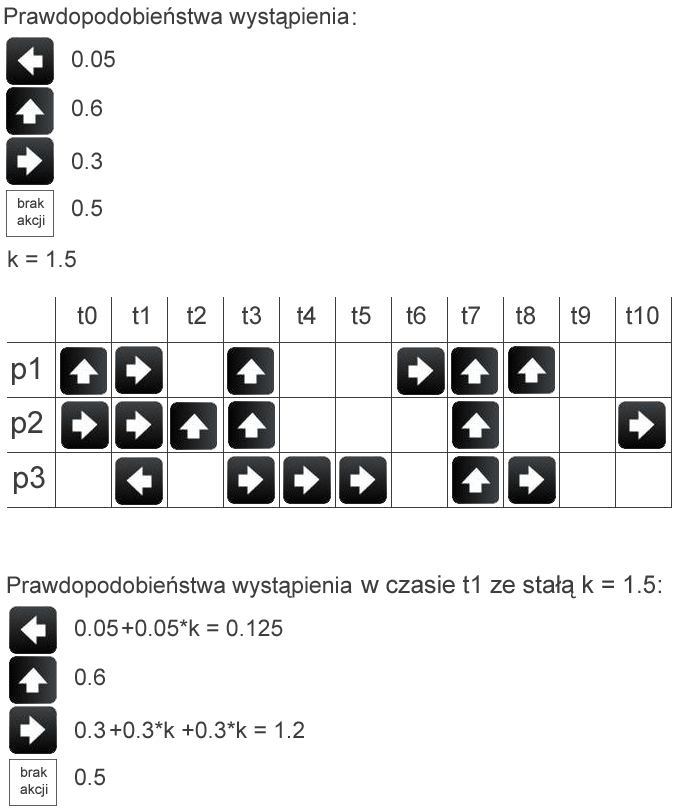
\includegraphics[width=5in]{obrazki/stat_cross.png}
		\caption{Krzyżowanie statystyczne.}
		\label{fig:krzyżowanie}
		\end{figure}

	\end{par}
	\item
	{\bf Aktualna pozycja gracza.}
	\begin{par}
		O ile poprzednie rozwiązanie dawało większą swobodę ruchu po mapie, to było jednak mało optymalne pod względem osiągania szybko dobrych wyników.
		Jeśli założymy iż akcje przechowywane w chromosomie mają być aktywowane w momencie osiągnięcia przez gracza danej pozycji na osi X mapy, wówczas uprościmy cały mechanizm krzyżowania (już nie musimy szukać punktów wspólnych, gdyż dwa dowolne indeksy w obu tablicach $i,j$ gwarantują nam takie samo położenie gracza na mapie gdy $i=j$.
		Oprócz tego przy założeniu że planszę da się rozwiązać poruszając się tylko w prawo upraszcza to większość operacji w algorytmie.
		Innym udogodnieniem będzie uproszczenie samego typu przechowywanych danych. Ponieważ rezygnujemy z postojów i ruchu w lewo, równie dobrze możemy zrezygnować z tablicy przechowującej te informacje.

		\begin{par}
		\begin{figure}[!h]
		\centering
		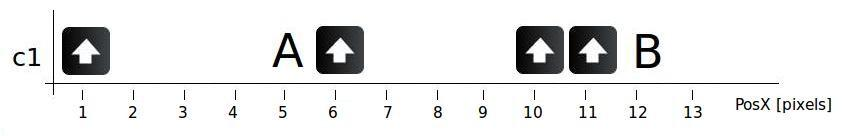
\includegraphics[width=\textwidth]{obrazki/sterowanie2.jpg}
		\caption{Sterowanie względem pozycji gracza.}
		\label{fig:sterowanie2}
		\end{figure}
		\end{par}

		To podejście posiada jednak kilka poważnych wad i wymaga pewnych ograniczających założeń.
		Plansza musi być ukierunkowana, i być rozwiązywalna przy ciągłym ruchu w określonym kierunku.
		Jest to rozwiązanie działające jedynie dla bardzo wąskiej grupy gier platformowych (np. wspomniane wcześniej Super Mario Brothers).
		Przeniesienie systemu do zastosowania w grze platformowej o nieco innym schemacie ruchu (np. rozwiązywania labiryntu) może okazać się trudne i wymagające dużych zmian w samym algorytmie.
		Jeśli chcemy tego uniknąć i traktować system bardziej ogólnie, lepiej jest skorzystać z pierwszego podejścia.
	\end{par}
	\end{enumerate}
	\FloatBarrier
\end{par}

\subsection{Diagram klas}
\begin{par}
	\begin{par}
	Diagram klas projektu przedstawiony został na rysunku \ref{fig:diagram_klas}.
	\end{par}
	\begin{figure}[!h]
	\centering
	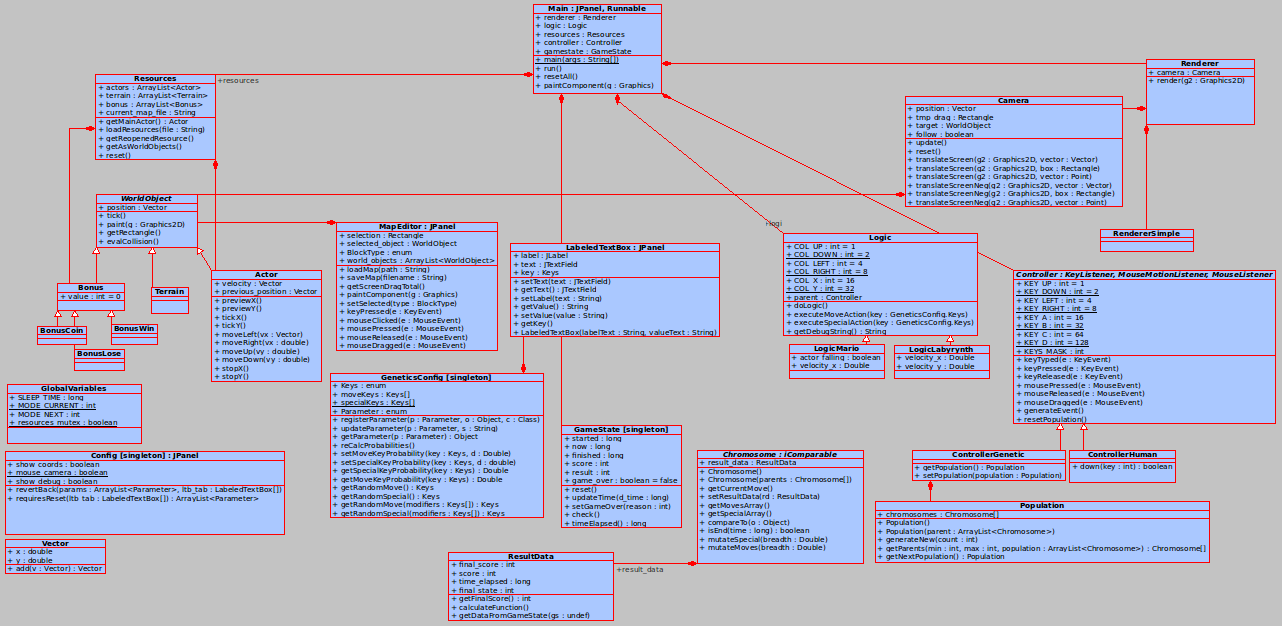
\includegraphics[width=\textwidth]{obrazki/diagram_klas.png}
	\caption{Diagram Klas.}
	\label{fig:diagram_klas}
	\end{figure}
\end{par}


